% !TeX root = ../proyecto.tex

\chapter{Entorno de Pruebas}\label{ch:entorno_de_pruebas}
En este capítulo se describe el entorno experimental empleado para evaluar los algoritmos propuestos.
Se detallan los conjuntos de datos utilizados, el diseño de los experimentos, el procedimiento de ejecución y las métricas de evaluación.
Asimismo, se explica cómo se presentan y visualizan los resultados obtenidos.


\section{Datasets utilizados}\label{sec:datasets}
En el aprendizaje profundo, los datasets son colecciones de datos etiquetados o no etiquetados que se utilizan para
entrenar modelos.
Estos conjuntos de datos contienen ejemplos organizados que representan la entrada para el modelo y, en muchos casos,
también las etiquetas correspondientes que indican la salida deseada.
Los datasets varían en tamaño, calidad y tipo, dependiendo de la tarea a resolver, como la clasificación de imágenes,
el reconocimiento de patrones o la predicción de series temporales.


A continuación, se van a explicar cada uno de los Datasets que se han utilizado en el desarrollo del proyecto.

\subsection{Rock, Paper, Scissors (Piedra, Papel, Tijera)}\label{subsec:rock-paper-scissors}
\textbf{Rock, Paper, Scissors}~\cite{RockPaperScissors} es un conjunto de datos creado por Laurence Moroney
que se utiliza para la clasificación de imágenes de manos representando los gestos de `piedra', `papel' y `tijeras'.

\begin{figure}[htp]
    \centering
    \begin{subfigure}[t]{0.3\textwidth}
        \centering
        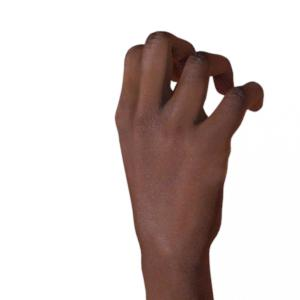
\includegraphics[width=\linewidth]{imagenes/dataset_examples/rock.jpg}
        \caption*{Rock}
    \end{subfigure}
    \begin{subfigure}[t]{0.3\textwidth}
        \centering
        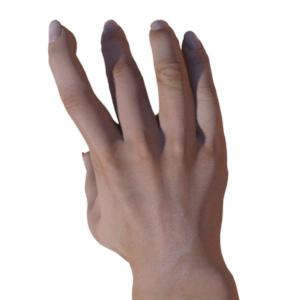
\includegraphics[width=\linewidth]{imagenes/dataset_examples/paper.jpg}
        \caption*{Paper}
    \end{subfigure}
    \begin{subfigure}[t]{0.3\textwidth}
        \centering
        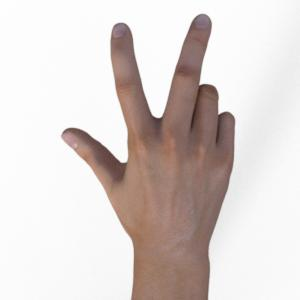
\includegraphics[width=\linewidth]{imagenes/dataset_examples/scissors.jpg}
        \caption*{Scissors}
    \end{subfigure}
    \caption{Ejemplos de imágenes del dataset Rock, Paper, Scissors}
    \label{fig:ejemplos-rps}
\end{figure}

En la figura~\ref{fig:ejemplos-rps} se han mostrado una imagen de cada una de las clases del dataset Rock, Paper, Scissors,
para que se pueda observar la similitud entre las distintas clases.

\subsubsection{Estructura del Dataset}
El conjunto de datos contiene aproximadamente 2,500 imágenes, distribuidas en tres categorías: piedra, papel y tijeras.
Las imágenes están en color y tienen un tamaño de 300x300 píxeles.

\begin{figure}[ht]
    \centering
    \begin{forest}mydirstyle
        [RPS
            [train
                    [rock
                            [image1.jpg]
                            [image2.jpg]
                            [\dots]
                    ]
                    [paper
                            [image1.jpg]
                            [image2.jpg]
                            [\dots]
                    ]
                    [scissors
                            [image1.jpg]
                            [image2.jpg]
                            [\dots]
                    ]
            ]
            [test (originalmente valid)
                [rock]
                    [paper]
                    [scissors]
            ]
            [valid (originalmente test)
                [rock]
                    [paper]
                    [scissors]
            ]
        ]
    \end{forest}
    \caption{Estructura de carpetas del dataset Rock, Paper, Scissors}
    \label{fig:estructura-rps}
\end{figure}


Como se puede observar en la Figura~\ref{fig:estructura-rps}, las imágenes están organizadas en directorios según su función en el entrenamiento
(entrenamiento, validación o prueba) y, dentro de cada partición, se dividen a su vez por clases del dataset.

\subsubsection{Formato de los Datos}
Las imágenes están en formato JPEG (\texttt{.jpg}).
Para su procesamiento, se han aplicado técnicas de preprocesamiento
adaptadas a los requerimientos del modelo.

\subsubsection{Uso del Dataset}
Este dataset se ha utilizado para evaluar el rendimiento del modelo en un problema de clasificación de imágenes con
múltiples clases, pero siendo un dataset sencillo y con un número de clases pequeño.
Además, permite explorar la eficacia de los algoritmos meméticos en un entorno más cercano al reconocimiento de objetos.

\subsubsection{Correcciones en la División de Datos}
Según la nota observada en el README del dataset:
\begin{quote}
    \textit{Note: in the source, Laurence calls ``validation'' as the ``test'', and ``test'' the ``validation''.}
\end{quote}
se han renombrado las particiones de \texttt{test} y \texttt{valid} para que correspondan correctamente con sus
propósitos.

\subsubsection{Licencia y uso}
Este conjunto de datos se distribuye bajo la licencia
\textbf{Creative Commons Attribution 4.0 International (CC BY 4.0)}, lo que permite su uso, modificación y distribución
con la condición de otorgar el crédito adecuado a los creadores originales.


\subsection{\texttt{PAINTING} (Art Images: Drawing/Painting/Sculptures/Engravings)}\label{subsec:painting}
El dataset \textbf{Art Images: Drawing/Painting/Sculptures/Engravings} es una colección de aproximadamente 9,000
imágenes organizadas en cinco categorías de arte: dibujos, pinturas, esculturas, grabados y arte iconográfico.

\begin{figure}[htp]
    \centering
    \begin{subfigure}[t]{0.3\textwidth}
        \centering
        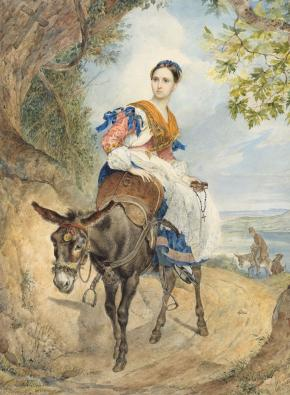
\includegraphics[width=\linewidth]{imagenes/dataset_examples/drawings.jpg}
        \caption*{Drawings}
    \end{subfigure}
    \begin{subfigure}[t]{0.3\textwidth}
        \centering
        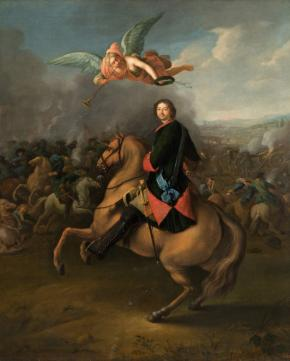
\includegraphics[width=\linewidth]{imagenes/dataset_examples/painting.jpg}
        \caption*{Painting}
    \end{subfigure}
    \begin{subfigure}[t]{0.3\textwidth}
        \centering
        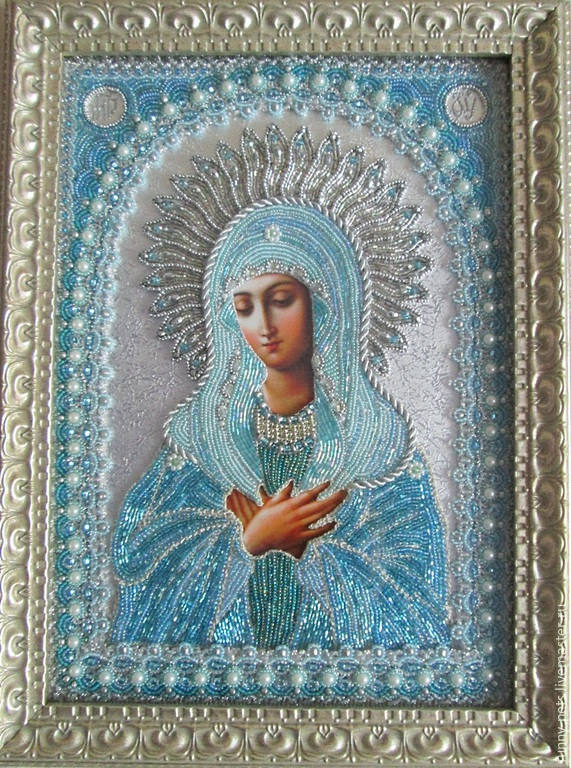
\includegraphics[width=\linewidth]{imagenes/dataset_examples/iconography.jpg}
        \caption*{Iconography}
    \end{subfigure}
    \begin{subfigure}[t]{0.3\textwidth}
        \centering
        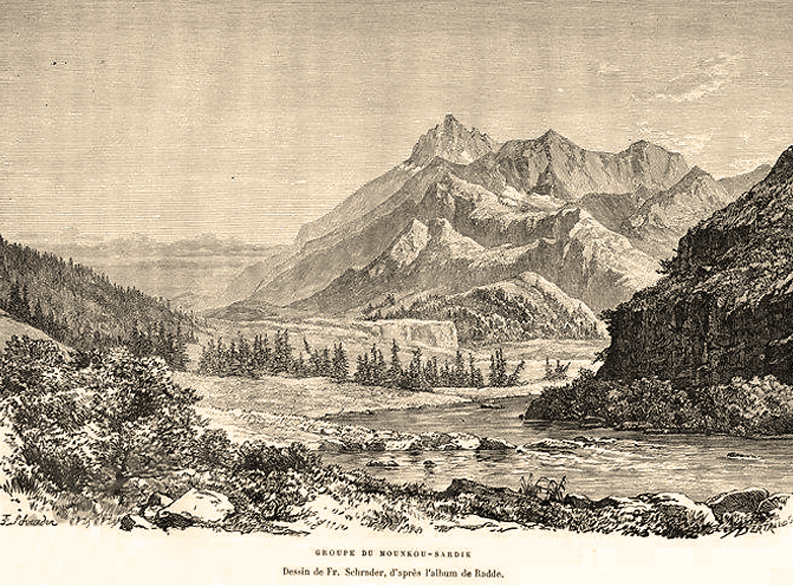
\includegraphics[width=\linewidth]{imagenes/dataset_examples/engraving.jpg}
        \caption*{Engraving}
    \end{subfigure}
    \begin{subfigure}[t]{0.3\textwidth}
        \centering
        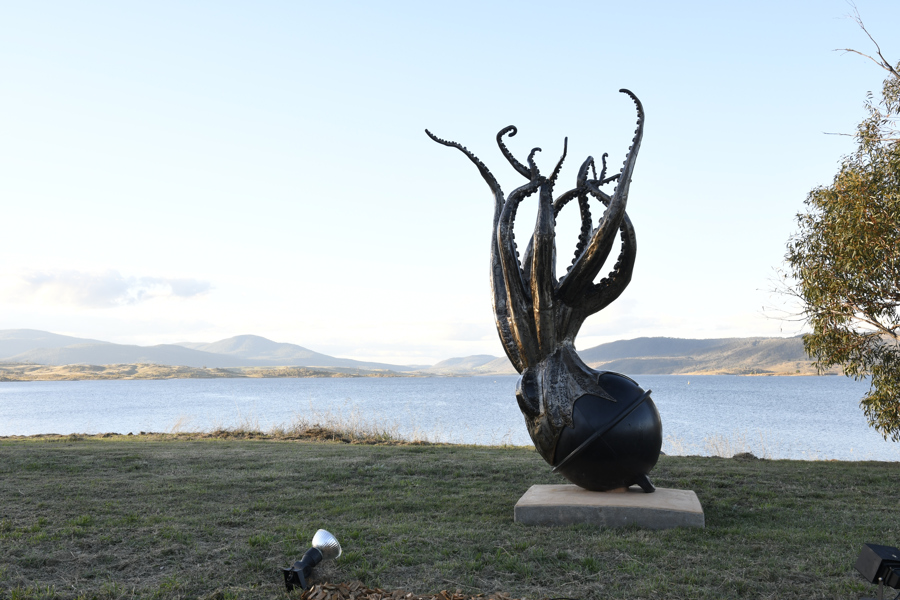
\includegraphics[width=\linewidth]{imagenes/dataset_examples/sculpture.jpg}
        \caption*{Sculpture}
    \end{subfigure}
    \caption{Ejemplos de clases en el dataset \texttt{PAINTING}}
    \label{fig:ejemplos-painting}
\end{figure}

En la figura~\ref{fig:ejemplos-painting} se han mostrado una imagen de cada una de las clases del dataset \texttt{PAINTING},
para que se pueda observar la variabilidad de las imágenes.

\subsubsection{Estructura del Dataset}
\begin{figure}[ht]
    \centering
    \begin{forest}mydirstyle
        [Dataset
            [Train (originalmente training\_set)
                [drawings
                            [image1.jpg]
                            [image2.jpg]
                            [\dots]
                    ]
                    [paintings
                            [image1.jpg]
                            [image2.jpg]
                            [\dots]
                    ]
                    [sculptures]
                    [engravings]
                    [iconography]
            ]
            [Test (originalmente validation\_set)
                [drawings]
                    [paintings]
                    [sculptures]
                    [engravings]
                    [iconography]
            ]
        ]
    \end{forest}
    \caption{Estructura de carpetas del dataset \texttt{PAINTING}}
    \label{fig:estructura-painting}
\end{figure}

Como se puede observar en la Figura~\ref{fig:estructura-painting}, las imágenes están organizadas en directorios según su categoría artística,
que en este caso corresponden a las distintas clases del dataset, previamente divididas en conjuntos de entrenamiento y prueba.

\subsubsection{Formato de los Datos}
Todas las imágenes están en formato JPEG (\texttt{.jpg}) y presentan variaciones en resolución y dimensiones.
Se han aplicado técnicas de preprocesamiento para homogenizar las características de las imágenes.

\subsubsection{Uso del Dataset}
Este dataset se ha utilizado para entrenar y evaluar modelos de clasificación de imágenes en un entorno diferente al
RPS\@.
Con este dataset, se ha comprobado el funcionamiento para evaluar los algoritmos con un dataset un poco mas complejo
que el RPS, con un par de clases más y con un número mayor de imágenes.

\subsubsection{Correcciones en la División de Datos}
Observando los tamaños de la división de los datos, y teniendo en cuenta que la divisón de los datos suele ser en train
y test, se ha decidido por renombrar las particiones de \texttt{valid} por \texttt{test} para que corresponda
correctamente con su propósito.
Y el set de validation lo he obtenido separando el set de train, normalmente haciendo una división 80\% test y 20\%
valid.

\subsubsection{Acceso al Dataset}
Inicialmente, el dataset se descargó desde Kaggle~\cite{OriginalArtImages}

Sin embargo, debido a la presencia de archivos innecesarios y algunas imágenes corruptas, se opta por una versión
limpia disponible en Kaggle~\cite{CleanedArtImages}.

\subsubsection{Licencia y Uso}
Antes de su uso, se revisaron los términos y condiciones establecidos en la página de Kaggle para asegurar el
cumplimiento con las licencias y restricciones aplicables.

\subsection{Comparación entre datasets}\label{subsec:comparacion-entre-datasets}
Gracias a la tabla~\ref{tab:resumen-datasets} que con las características más relevantes de los datasets utilizados,
permite entender mejor la complejidad relativa de cada conjunto y cómo pueden influir en el comportamiento de los algoritmos:

\begin{table}[htp]
    \centering
    \resizebox{\textwidth}{!}{
        \begin{tabular}{|l|c|c|c|c|}
            \hline
            \textbf{Dataset}      & \textbf{Nº Imágenes} & \textbf{Nº Clases} & \textbf{Formato} & \textbf{Tamaño Imagen} \\
            \hline
            Rock, Paper, Scissors & \textasciitilde2.500 & 3                  & JPG              & 300×300 px             \\
            PAINTING              & \textasciitilde9.000 & 5                  & JPG              & Variable               \\
            \hline
        \end{tabular}
    }
    \caption{Resumen comparativo de los datasets utilizados}
    \label{tab:resumen-datasets}
\end{table}

La selección de estos dos datasets responde a la necesidad de evaluar los algoritmos meméticos en distintos niveles de complejidad.
El dataset \textbf{Rock, Paper, Scissors} se utilizó en las primeras fases del proyecto como punto de partida,
ya que ofrecía un entorno sencillo y controlado, con un número reducido de clases y una estructura equilibrada.
Esto permite desarrollar las bases del sistema y probar las primeras versiones de los algoritmos de manera más ágil y con menor complejidad computacional.

Por su parte, el dataset \textbf{PAINTING} se empleó posteriormente para validar el comportamiento de los algoritmos en un entorno más exigente.
Al incluir cinco categorías de arte con distintos estilos visuales, este conjunto introdujo una mayor variabilidad tanto semántica como estructural,
lo que permite evaluar la robustez y capacidad de generalización de las soluciones desarrolladas.


\section{Diseño de los experimentos}\label{sec:diseño-de-los-experimentos}
La fase experimental se organiza en varias etapas.
Inicialmente se opta por un dataset simple (\textit{Rock, Paper, Scissors}) para validar el funcionamiento general del sistema.
Posteriormente, se realizan pruebas con datasets más exigentes.
Los experimentos se repiten utilizando diferentes porcentajes iniciales de datos (10\%, 25\%, 50\% y 75\%)
para estudiar cómo afecta la cantidad de datos seleccionados al rendimiento del modelo.

Con el fin de asegurar la consistencia entre ejecuciones experimentales, se aplican las medidas de control de reproducibilidad
descritas en el \hyperref[sec:consideraciones-de-optimizacion]{Apartado~\ref*{sec:consideraciones-de-optimizacion}}.
Esto permite comparar algoritmos en condiciones homogéneas, evitando variaciones indeseadas causadas por componentes aleatorios del entorno de ejecución.

En cada prueba, se realizan 5 ejecuciones en paralelo, cada una utilizando una semilla distinta.
Esta estrategia permite obtener resultados promedio más robustos frente a la aleatoriedad del proceso evolutivo, asegurando una mayor fiabilidad estadística.

Los apartados siguientes explican con mayor detalle el procedimiento adoptado para llevar a cabo dichas ejecuciones.


\section{Procedimiento de Ejecución y Evaluación}\label{sec:procedimiento-de-ejecucion-y-evaluacion}
Para garantizar la consistencia y objetividad en la comparación entre algoritmos, se diseñan un procedimiento experimental sistemático y replicable.
Cada ejecución se realizó bajo las mismas condiciones computacionales y utilizando los mismos parámetros base,
salvo en aquellos casos en que se deseaba estudiar una variación concreta, como los distintos porcentajes iniciales o el uso de metaheurísticas con porcentajes libres.

\subsection{Métricas de Evaluación}\label{sec:metricas-de-evaluacion}
Para evaluar el rendimiento de los modelos se utilizaron métricas estándar como \textbf{accuracy}, \textbf{precisión}, \textbf{recall} y \textbf{F1-score},
calculadas sobre el conjunto de validación tras cada evaluación.
Para una definición formal de estas métricas, véase el \hyperref[sec:metricas-evaluacion]{Apartado~\ref*{sec:metricas-evaluacion}}.

Estas métricas se calcularon utilizando las funciones de \texttt{scikit-learn}, a partir de las predicciones del modelo y las etiquetas
reales correspondientes a los subconjuntos de imágenes seleccionados por cada algoritmo.

\subsection{Evaluaciones por Ejecución}\label{sec:evaluaciones-por-ejecucion}
Se buscó un equilibrio entre la cantidad de evaluaciones y el tiempo de ejecución, permitiendo una exploración suficiente del espacio de soluciones sin comprometer la eficiencia computacional.
Por ello, cada algoritmo se configura para realizar un máximo de 100 evaluaciones por ejecución,
independientemente del tipo de algoritmo utilizado, con el fin de mantener la equidad comparativa.

Cada evaluación consiste en generar un subconjunto de datos, entrenar el modelo correspondiente (ResNet50 o MobileNetV2),
y calcular su \textit{fitness} de acuerdo con las métricas mencionadas.

El número de evaluaciones sin mejora también se monitoriza para aplicar criterios de parada anticipada,
explicados previamente en el \hyperref[sec:consideraciones-de-optimizacion]{Apartado~\ref*{sec:consideraciones-de-optimizacion}},
reduciendo así el tiempo computacional en caso de estancamiento.

\subsubsection{Visualización de resultados}\label{subsec:visualizacion-de-resultados}
Para facilitar la comparación entre algoritmos, a lo largo de este capítulo se incluyen representaciones gráficas de los
resultados obtenidos mediante \textbf{boxplots} y \textbf{barplots}.
Ambos tipos de gráficos permiten visualizar el comportamiento global de cada algoritmo a partir de múltiples ejecuciones con distintas semillas.

\textbf{Los boxplots} (diagramas de caja) muestran la distribución estadística de los valores obtenidos.
En la Figura~\ref{fig:boxplot-explicado} se presenta un ejemplo anotado que ilustra las distintas partes de este tipo de gráfico.
La línea central de la caja representa la \textbf{mediana},
mientras que los bordes inferior y superior corresponden al \textbf{primer cuartil} (Q1) y \textbf{tercer cuartil} (Q3), respectivamente.
La diferencia entre ellos define el \textbf{rango intercuartílico} (\textit{IQR}), que contiene el 50\% central de los valores.
Las líneas que se extienden desde la caja (conocidas como \textit{bigotes}) alcanzan típicamente hasta 1.5 veces el IQR.
Los puntos que quedan fuera de ese rango se consideran \textbf{valores atípicos}, lo que permite detectar ejecuciones excepcionales.
Esta representación es especialmente útil para comparar la tendencia central, la dispersión y la estabilidad de los resultados obtenidos por los distintos algoritmos.

\begin{figure}[H]
    \centering
    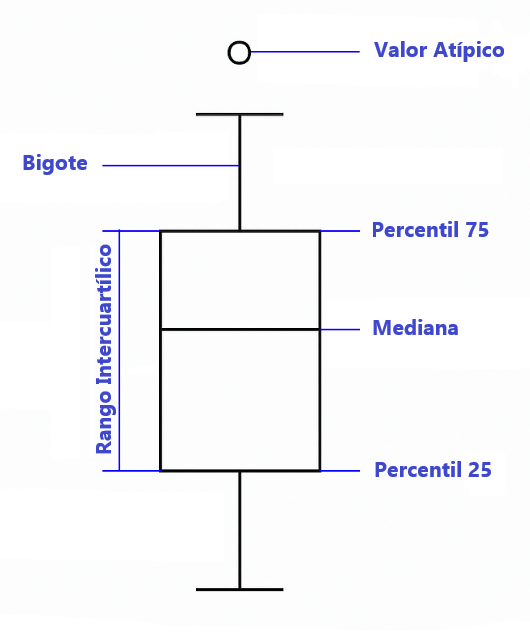
\includegraphics[width=0.45\textwidth]{imagenes/boxplot-explicado}
    \caption{Ejemplo de boxplot explicado.}
    \label{fig:boxplot-explicado}
\end{figure}

\textbf{Los barplots} (gráficos de barras), por su parte, se emplean para representar valores agregados como medias o proporciones,
y son útiles para observar cómo varía una métrica concreta entre distintos algoritmos, modelos o configuraciones.

\subsection{Repeticiones y Semillas}\label{sec:repeticiones-y-semillas}
Con el objetivo de obtener resultados estadísticamente significativos y reducir el efecto de la aleatoriedad,
cada configuración experimental se ejecuta 5 veces, utilizando 5 semillas distintas.
Los resultados presentados en las tablas y gráficos corresponden a la media de esas ejecuciones,
junto con medidas de dispersión cuando procede, como los boxplots.

Cabe destacar que, en el caso de los boxplots, en lugar de representar la media de las 5 ejecuciones por configuración,
se opta por incluir todos los valores individuales obtenidos con las distintas semillas.
Esta decisión permite visualizar una distribución más realista del comportamiento de cada algoritmo,
resaltando mejor la mediana, así como los valores máximos y mínimos alcanzados durante las ejecuciones.

\subsection{Tiempos de Ejecución}\label{sec:tiempos-de-ejecucion}
Cada evaluación implica entrenar un modelo desde cero, por lo que los tiempos de ejecución son considerables.
Por ejemplo, una ejecución completa con 100 evaluaciones puede tardar entre 30 minutos y 2 horas,
dependiendo del algoritmo y del modelo utilizado.

Los algoritmos más complejos, como el memético o las versiones con reinicio poblacional,
requieren un mayor tiempo de ejecución debido a las operaciones adicionales de mejora local o regeneración de población.


\section{Nomenclatura simplificada de los algoritmos}
Para facilitar la lectura de las tablas y gráficos presentados a lo largo de este trabajo,
se opta por utilizar abreviaciones consistentes para referirse a los algoritmos implementados.
Estas abreviaciones permiten condensar la información visualmente sin perder la claridad en la interpretación de los resultados.

La correspondencia entre el nombre completo de cada algoritmo y su abreviatura se muestra en la Tabla~\ref{tab:nombres-algoritmos}.

\begin{table}[htp]
    \centering
    \begin{tabular}{ll}
        \toprule
        \textbf{Nombre Completo del Algoritmo}                 & \textbf{Abreviatura} \\
        \midrule
        Aleatorio (Random Search)                              & RS                   \\
        Búsqueda Local (Local Search)                          & LR                   \\
        Búsqueda Local Libre                                   & LR-F                 \\
        Algoritmo Genético                                     & GEN                  \\
        Genético con Cruce Ponderado (Weighted Crossover)      & WC                   \\
        Genético con Cruce Ponderado Libre                     & WC-F                 \\
        Genético con Reinicio Poblacional (Population Restart) & PR                   \\
        Algoritmo Memético                                     & MEM                  \\
        Algoritmo Memético Libre                               & MEM-F                \\
        \bottomrule
    \end{tabular}
    \caption{Nomenclatura simplificada de los algoritmos.}
    \label{tab:nombres-algoritmos}
\end{table}

A partir de este punto, todas las tablas y gráficos del documento utilizarán estas abreviaturas para referirse a los algoritmos,
mejorando la legibilidad de los resultados y facilitando la interpretación de las comparativas entre métodos.
